\chapter{Research}\label{research}
% This chapter, or series of chapters, delves into all technical details that are
% required to \emph{prove} your scientific hypothesis.
% It should be sufficiently detailed and precise in order for any fellow computing scientist student to be able to \emph{repeat}
% your research and therewith establish the same results / conclusions that you have obtained.
% Please note that, in order to improve readability of your thesis, you can put a part of this information also in one or
% more appendices (see Appendix \ref{appendix}).

In this section we will explain the technical details of our DistilBERT model. First, we will justify which libraries and framework we used for our model. Second, we will showcase how we have implemented the libraries in python to create our model. Afterwards, we will analyze our dataset, consisting of malicious and benign domains. Lastly, we will demonstrate the results of our model. The python notebook code is accessible in \ref{appendix}.

\section{System Architecture}
To build and train our DistilBERT model, we used the ktrain library \cite{maiya2020ktrain}. Ktrain is a lightweight open source wrapper for the deep learning library TensorFlow Keras \cite{chollet2015keras}. According to the authors, it helps to build, train and deploy neural networks in a more accessible and easier way. Ktrain allows you to easily estimate an optimal learning rate for your model given a learning rate finder.\\\\
For data analysis on our dataset, we use the open source scikit-learn library \cite{sklearn_api}. It is a simple and efficient tool to predict and analyze data, built on NumPy, SciPy and matplotlib.


\section{Datasets}
This paper uses two open datasets to make the research reproducible. The Tranco one million domains \cite{Tranco} are used for benign, non DGA, domains. Tranco is a research-oriented top sites ranking dataset that is hardened against manipulation. Most researchers \cite{Antonakakis}\cite{Lison}\cite{Highnam}\cite{TRAN20182401} rely on popularity rankings such as the Alexa top one million domain list. However, the Tranco paper \cite{Tranco} finds out that it is trivial for an adversary to manipulate the composition of these lists. The list of Alexa top one million can be altered by as little as a single HTTP request by adversaries. 
\\
Therefore, the Tranco paper comes up with an one million domain list that is hardened against these manipulations. This is the list we use for our DGA domain detector. We only use a fourth of the domains in the 1 million Tranco list, totalling $200000$ benign domains.\\\\
For the DGA malicious domains, we use the UMUDGA dataset \cite{UMUDGA}. UMUDGA is a dataset for profiling DGA-based botnets. It contains 37 notorious distinct malware variants generated domain lists. For our model, we have opted out for approximately $5000$ domain lists per malware variant. Our DGA domains totals $184765$. Combined we have a total of $384765$ domains in our dataset, with a proportion of 52\% between benign and DGA domains.

\section{DistilBERT Detector}
To prepare our dataset for the detector, we first separate our dataset into input (X) and output (y) columns.  Then, we use the sklearn library function \textit{train\_test\_split(X,y, test\_size, random\_state)}, which splits our dataset into a random train and test (validation) dataset. This function uses a random state, which accepts an integer seed to control the shuffling applied to the data before the split. The test\_size indicates the percent of the dataset that will be allocated to the test set. For our model, the proportion between train and test date is 25\% and 75\% respectively.\\\\
The ktrain library wraps pre-trained, fast and easy to use models that can be applied to our text data. The text classification model that we will use for our detector is the DistilBERT \cite{Sanh2019DistilBERTAD} model. As mentioned in the introduction, it is a distilled version of BERT, that reduces BERT by 40\%, while still retaining 97\% of its language understanding capabilities and being 60\% faster. DistilBERT is pre-trained on the same data as BERT \cite{ColBERT}. In our model we use the English uncased base pre-trained DistilBERT model. The texts in the model are lowercase and tokenized using WordPiece \cite{WordPiece} and a vocabulary size of $30000$. The DistilBERT model is trained on 8, 16 GB V100 for 90 hours. We use this model to preprocess our training and test data using the ktrain wrapper. 


\subsection{Learning Rate}
We wrap our preprocessed training and test dataset into the \textit{ktrain.Learner} object using the \textit{ktrain.get\_learner(model, train\_data, val\_data, batch\_size)} function. We use a batch size of six for our network. The batch size is the number of samples that will be passed through to the neural network.\\\\
\\The important hyperparameters that we have to set for our neural network is the learning rate. To properly train a neural network, we have to minimize the loss function. If the learning rate is too high, training will not be minimized. However, if the learning rate is too low, training will be slow or can stall. 
To have an optimal learning rate for our model, we can simulate the training by starting with a low training rate and gradually increasing it. As written by Leslie Smith \cite{Learning_Rate} in his paper, he indicates that when plotting the learning rate versus the loss, a good choice for training is the maximal learning rate associated with a still falling loss. This is referred to by Smith as an LR Range Test, or as an LR Finder. The LR Finder can be executed in ktrain as well using the function \textit{lr\_find()} and produce a plot with the \textit{lr\_plot()} function. We can select the maximal learning rate where the loss is still falling prior to divergence in the plot.\\\\ 
A number of studies have shown that by varying the learning rate during training can improve performance to a neural model in terms of both loss minimization and better validation accuracy. A learning rate schedule, such as the 1cycle learning rate schedule \cite{cycle_learning_rate} has benefits to the learning rate. Ktrain has a \textit{fit\_onecycle} function that employs the 1cycle policy. This policy increases for the first half of the training the learning rate from a base rate to a maximum rate, while decays the learning rate to a near-zero value for the second half of the training. Therefore, the maximum learning rate is set using the learning rate finder function mentioned above as well as using the 1cycle learning rate function to train our model.
After we have applied the \textit{lr\_find()} function on our model and plotted this with the \textit{lr\_plot()} function \ref{figure_lr}. We select the maximal learning rate where the loss is still falling prior to divergence. Therefore we choose $3^{e-5}$

\begin{figure}[!htb]
    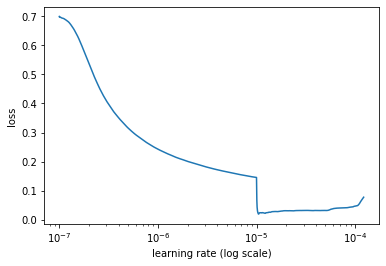
\includegraphics[width=10cm]{DistilBERT_detector_1}
    \caption{DistilBERT LR Range test result}
    \label{figure_lr}
\end{figure}
\pagebreak

\section{Metrics For Validation}
To measure our model performance, we calculate multiple metrics that are used commonly in machine learning research. To illustrate the metrics, we will use the following abbreviations: true positive (TP), true negative (TN), false positive (FP), false negative (FN), true positive rate (TPR) and false positive rate (FPR). The metrics are calculated as follows:

$${
            Precision = \frac{\sum TP}{\sum TP + \sum FP}
        }
$$

The precision metrics measures the ratio of correct positively labeled instances to all positively labeled instances.

$${
            Recall = \frac{\sum TP}{\sum TP + \sum FN}
        }
$$

The recall metrics measures the ratio of correct positively labeled instances to all instances that should have been labeled positive.

$${
            F_1 = 2 \cdot \frac{Precision \cdot Recall}{Precision + Recall}
        }
$$

$F_1$ is the harmonic mean of Precision and Recall.
\pagebreak
$${
            TPR = \frac{\sum TP}{\sum TP + \sum FN}
        }
$$
\\True Positive Rate (TPR) is a synonym for Recall.

$${
            FPR = \frac{\sum FP}{\sum FP + \sum TN}
        }
$$
False Positive Rate (FPR) determines the rate of incorrectly identified labeled instances.
$${
            Accuracy = \frac{TP + TN}{TP + TN + FP + FN}
        }
$$
Accuracy is the fraction of predictions our model solved correctly.
\\\\
The receiving operating characteristics (ROC) curve is an evaluation metric for binary classification problems that plots TPR and FPR at various threshold values. It essentially separates the 'signal' from 'noise'. The ROC curve is a good metric to find out if our neural network is overfitting. The area under the curve (AUC) is an area under the ROC curve that compares ROC curves. Models whose predictions are 100\% wrong, have an AUC of 0.0, whereas models whose predictions are 100\% correct have an AUC of 1.0.

\section{Experiment}

This section evaluates the performance of our DistilBERT model. All operations are performed on a Google Cloud platform. We utilized the Google Colab Pro+ features, which gave us access to 1 V100 GPU, 53 GB of RAM and 8 CPU cores.\\\\ 
We have trained our model for 8 hours, 33 minutes and 13 seconds in 4 epochs. It had an accuracy of $0.9877$ for the train data and $0.9809$ for the test (validation) data. In figure \ref{figure_model} we can find our learner performance in each epoch on our train and validation data.
\begin{figure}[!htb]
    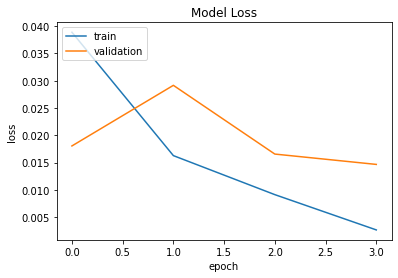
\includegraphics[width=10cm]{DistilBERT_detector_2}
    \caption{Calculating our training performance: loss of our model in each epoch for our train and validation dataset}
    \label{figure_model}
\end{figure}
\pagebreak
\\Whenever the model is trained, we have to cross-check the model with the test data. For that we can use the \textit{validate} function of the ktrain library. The results of our experiments are given in Table \ref{general_results}. We can observe that our model performed exceedingly well, having an accuracy of 99\%. Furthermore, both the benign and DGA domains, totalling $96192$, have an average of 99\%.\\\\
In order to find out how our model performed on each specific DGA family, we evaluated all 37 DGA families and benign domains to get their Precision, Recall and F1-score. The results of that experiment can be found in Table \ref{specific_results}. While evaluating the results, we are able to observe that our model has a better performance on non dictionary-based DGA than dictionary-based DGA families. Dictionary-based DGA families such as \textit{nymaim, matsnu, gozi} have a score lower than the average score of 99\%. A possible reason for this could be that our dataset has more non dictionary-based DGA families compared to dictionary-based DGA families. Our model has more training data on non dictionary-based DGA families, therefore our model is more bias towards them. Our model also seems to struggle more with short-length DGA domains, like \textit{proslikefan, pykspa} DGA families, that have a shorter domain name (URL) compared to other DGA families. This could be, because our DistilBERT model is pre-trained on long English sentences.\\\\  
We also evaluated the ROC-AUC score for our model. Our model has an ROC-AUC score of $0.9997$. This score surpassed the ROC-AUC score of previous research, such as \cite{Highnam} and \cite{Woodbridge}.


\begin{table}[!htb]
    \centering
    \begin{tabular}{llrll}
        \hline
                     & Precision & Recall & F1-score & Support \\ \hline
        benign       & 0.9955    & 0.9964 & 0.9964   & 50103   \\
        DGA          & 0.9961    & 0.9951 & 0.9956   & 46089   \\ \hline
        accuracy     &           &        & 0.9958   & 96192   \\
        macro avg    & 0.9957    & 0.9957 & 0.9957   & 96192   \\
        weighted avg & 0.9958    & 0.9958 & 0.9958   & 96192   \\ \hline
    \end{tabular}
    \caption{Results of our DistilBERT model, expressed in Precision, Recall and F1-score}
    \label{general_results}
\end{table}

\begin{table}[!htb]
    \rowcolors{2}{gray!25}{white}
    \centering
    \scalebox{0.85}{
        \begin{tabular}{l|l|llll}
            \hline
            nr & DGA          & Precision & \multicolumn{1}{r}{Recall} & F1-score        & Support \\ \hline
            1  & alureon      & 1.0000    & 0.9905                     & 0.9952          & 1268    \\
            2  & banjori      & 1.0000    & 1.0000                     & 1.0000          & 1283    \\
            3  & bedep        & 1.0000    & 0.9984                     & 0.9992          & 1248    \\
            4  & benign       & 1.0000    & 0.9964                     & 0.9982          & 50103   \\
            5  & ccleaner     & 1.0000    & 1.0000                     & 1.0000          & 1234    \\
            6  & chinad       & 1.0000    & 1.0000                     & 1.0000          & 1332    \\
            7  & corebot      & 1.0000    & 1.0000                     & 1.0000          & 1270    \\
            8  & cryptolocker & 1.0000    & 1.0000                     & 1.0000          & 1261    \\
            9  & dircrypt     & 1.0000    & 0.9951                     & 0.9976          & 1237    \\
            10 & dyre         & 1.0000    & 1.0000                     & 1.0000          & 1235    \\
            11 & fobber       & 1.0000    & 0.9952                     & 0.9976          & 1258    \\
            12 & gozi         & 1.0000    & \textbf{0.9873}            & \textbf{0.9936} & 1257    \\
            13 & kraken       & 1.0000    & 0.9958                     & 0.9979          & 1189    \\
            14 & locky        & 1.0000    & 0.9959                     & 0.9980          & 1230    \\
            15 & matsnu       & 1.0000    & \textbf{0.9821}            & \textbf{0.9910} & 1226    \\
            16 & murofet      & 1.0000    & 1.0000                     & 1.0000          & 1238    \\
            17 & necurs       & 1.0000    & 0.9983                     & 0.9992          & 1206    \\
            18 & nymaim       & 1.0000    & \textbf{0.9613}            & \textbf{0.9803} & 1188    \\
            19 & padcrypt     & 1.0000    & 0.9983                     & 0.9992          & 1191    \\
            20 & pizd         & 1.0000    & 1.0000                     & 1.0000          & 1182    \\
            21 & proslikefan  & 1.0000    & \textbf{0.9800}            & \textbf{0.9900} & 1298    \\
            22 & pushdo       & 1.0000    & 0.9917                     & 0.9958          & 1198    \\
            23 & pykspa       & 1.0000    & \textbf{0.9848}            & \textbf{0.9924} & 1253    \\
            24 & qadars       & 1.0000    & 0.9992                     & 0.9996          & 1298    \\
            25 & qakbot       & 1.0000    & 1.0000                     & 1.0000          & 1213    \\
            26 & ramdo        & 1.0000    & 1.0000                     & 1.0000          & 1270    \\
            27 & ramnit       & 1.0000    & 0.9968                     & 0.9984          & 1250    \\
            28 & ranbyus      & 1.0000    & 1.0000                     & 1.0000          & 1247    \\
            29 & rovnix       & 1.0000    & 0.9944                     & 0.9972          & 1249    \\
            30 & shiotob      & 1.0000    & 0.9976                     & 0.9988          & 1264    \\
            31 & simda        & 1.0000    & 0.9961                     & 0.9980          & 1272    \\
            32 & sisron       & 1.0000    & 1.0000                     & 1.0000          & 1215    \\
            33 & suppobox     & 1.0000    & 1.0000                     & 1.0000          & 1252    \\
            34 & symmi        & 1.0000    & 1.0000                     & 1.0000          & 1252    \\
            35 & tempedreve   & 1.0000    & 0.9874                     & 0.9937          & 1282    \\
            36 & tinba        & 1.0000    & 0.9992                     & 0.9996          & 1296    \\
            37 & vawtrak      & 1.0000    & 0.9918                     & 0.9959          & 1220    \\
            38 & zeus-newgoz  & 1.0000    & 0.9992                     & 0.9996          & 1237   
        \end{tabular}
    }
    \caption{Results of our DistilBERT model on each distinct DGA family, expressed in Precision, Recall and F1-score. The }
    \label{specific_results}
\end{table}

% \section{Comparison}
% To further evaluate our model, we compare our results to previous models. Notoriously, dictionary based DGA families such as \textit{matsnu, suppobox and gozi}, are hard to classify. Hence, the performance of most models are low on these DGA families. Therefore, we compare the results of 5 different deep learning architectures, including our model to these three DGA families. The results of the comparison can be seen in Table \ref{comparison_results}. We can see that our DistilBERT model outperforms the previous models by a large margin. 

% \begin{table}[!htb]
%     \centering
%     \begin{tabular}{l|lllll}
%         \hline
%         Model                  & Precision       & Recall          & F1-score        & Accuracy        & AUC             \\ \hline
%         ANN \cite{}            & 0.9077          & 0.8250          & 0.8644          & 0.8566          & 0.9290          \\
%         CNN                    & 0.9730          & 0.9473          & 0.9600          & 0.9593          & 0.9919          \\
%         LSTM \cite{Woodbridge} & 0.9675          & 0.9627          & 0.9651          & 0.9653          & 0.9932          \\
%         Bilbo \cite{Highnam}   & 0.9766          & 0.9557          & 0.9660          & 0.9656          & 0.9944          \\
%         DistilBERT             & \textbf{0.9989} & \textbf{0.9898} & \textbf{0.9948} & \textbf{0.9898} & \textbf{0.9997} \\ \hline
%     \end{tabular}
%     \caption{Comparing the results of six different deep learning architectures for three dictionary-based DGA families: matsnu, gozi and suppobox. The best results are bold.}
%     \label{comparison_results}
% \end{table}
